\indent Por consiguiente, mostraremos buenos y malos casos para nuestro algoritmo, y a su vez, daremos el tiempo estimado 
seg\'un la complejidad del algoritmo calculada anteriormente.\\

Luego de varios experimentos, pudimos llegar a la conclusi\'on que uno de los tipos de casos que resulta m\'as beneficioso para nuestro algoritmo
es en el cual el rollo de cable llega a cubrir y conectar todas las estaciones.\\

Para llegar a dicha conclusi\'on trabajamos con un total de 100 instancias y un n entre 1 y 1000000 obtuvimos que nuestro
algoritmo finaliza lo solicitado demorando 184 milisegundos.\\

Para una mayor observacion desarrollamos el siguiente grafico con las instancias:\\

\vspace*{0.3cm} \vspace*{0.3cm}
  \begin{center}
 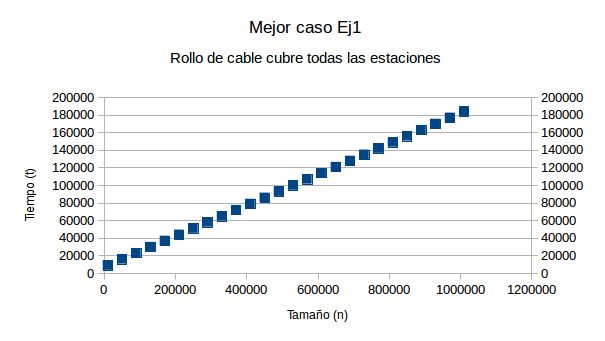
\includegraphics[scale=0.8]{./EJ1/mejorcasoej1.png}
  \end{center}
  \vspace*{0.3cm}


Si a esto lo dividimos por la complejidad propuesta obtenemos:\\

\vspace*{0.3cm} \vspace*{0.3cm}
  \begin{center}
 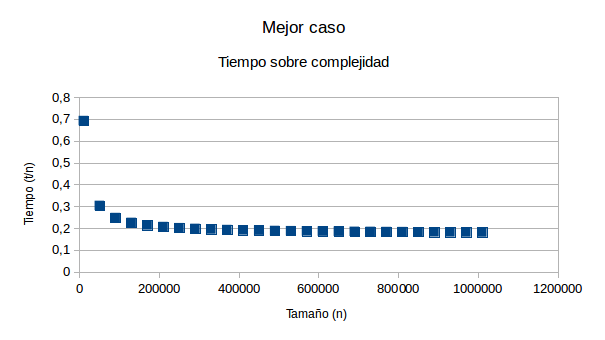
\includegraphics[scale=0.8]{./EJ1/mejorcasoej11.png}
  \end{center}
  \vspace*{0.3cm}

 Para realizar esta divisi\'on realizamos un promedio con el mismo input de aproximadamente 20 corridas
tanto para la complejidad como para nuestro algoritmo y una vez calculado dicho promedio de ambas cosas realizamos la divisi\'on para
obtener resultados m\'as consisos.\\ 

  
  
A continuaci\'on, adjuntamos una tabla con los considerados “mejor” caso que nos parecieron m\'as relevantes

\begin{table}[H]

    \begin{tabular}{ | l | l |l |}
    \hline
		Tamaño($n$) & Tiempo($t$) & \textbf{$t /n$}  \\ \hline
610000 & 114000 & 0,186 \\ \hline
650000 & 121000 & 0,185 \\ \hline
690000 & 128000 & 0,185 \\ \hline
730000 & 135000 & 0,184 \\ \hline
770000 & 142000 & 0,184 \\ \hline
810000 & 149000 & 0,183 \\ \hline
850000 & 156000 & 0,183 \\ \hline
890000 & 163000 & 0,183 \\ \hline
930000 & 170000 & 0,182 \\ \hline
970000 & 177000 & 0,182 \\ \hline
1010000 & 184000 & 0,182 \\ \hline

\textbf{Promedio} & & 0.217 \\ \hline

    \end{tabular}
\end{table}

Dando un \textbf{promedio igual a 0.217 }\\

Luego, uno de los peores casos para nuestro algoritmo es en el cual el rollo de cable no llega a cubrir ninguna distancia entre ciudades.\\

Para llegar a dicha conclusi\'on trabajamos con un total de 100 instancias y un n entre 1 y 1000000 obtuvimos que nuestro
algoritmo finaliza lo solicitado demorando 224 milisegundos.\\

\vspace*{0.3cm} \vspace*{0.3cm}
  \begin{center}
 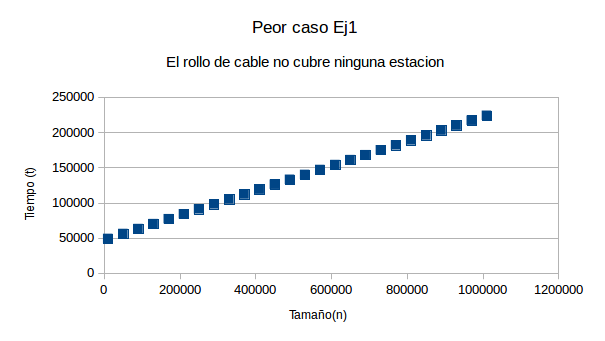
\includegraphics[scale=0.8]{./EJ1/peorcasoej1.png}
  \end{center}
  \vspace*{0.3cm}

Si a esto lo dividimos por la complejidad propuesta obtenemos:\\

\vspace*{0.3cm} \vspace*{0.3cm}
  \begin{center}
 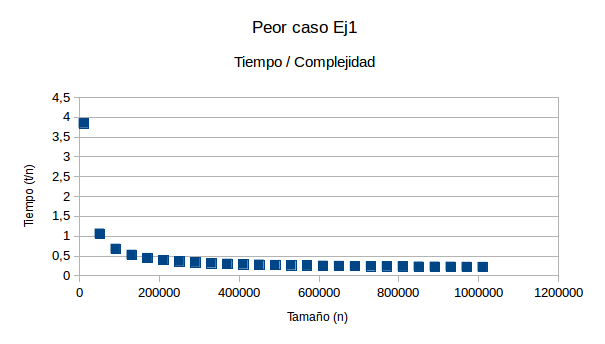
\includegraphics[scale=0.8]{./EJ1/peorcasoej11.png}
  \end{center}
  \vspace*{0.3cm}
  
  Para realizar esta experimentaci\'on nos parecio acorde, realizar un promedio con el mismo input de aproximadamente 20 corridas
tanto para la complejidad como para nuestro algoritmo y una vez calculado dicho promedio de ambas cosas realizamos la divisi\'on para
obtener resultados m\'as relevantes.\\ 


La informaci\'on de los 10 datos mas relevantes referiendonos al peor caso fueron:

\begin{table}[H]

    \begin{tabular}{ | l | l |l |}
    \hline
	Tamaño($n$) & Tiempo($t$) & \textbf{$t /n$}  \\ \hline
610000 & 154000 & 0,251 \\ \hline
650000 & 161000 & 0,247 \\ \hline
690000 & 168000 & 0,243 \\ \hline
730000 & 175000 & 0,239 \\ \hline
770000 & 182000 & 0,236 \\ \hline
810000 & 189000 & 0,233 \\ \hline
850000 & 196000 & 0,230 \\ \hline
890000 & 203000 & 0,227 \\ \hline
930000 & 210000 & 0,225 \\ \hline
970000 & 217000 & 0,223 \\ \hline
1010000 & 224000 & 0,221 \\ \hline
    \textbf{Promedio} & & 0.469 \\ \hline

    \end{tabular}
\end{table}

Dando un \textbf{promedio igual a 0.469} \\

Aqu\'i, podemos observar como la cota de complejidad del algoritmo y la de dicho caso tienden al mismo valor con el paso del tiempo.\\